\documentclass[crop,tikz]{standalone}

\usepackage{pgfplots}
\tikzset{>=latex}

\colorlet{green}{black!40!green}

\pgfplotsset{
  every non boxed x axis/.append style={
    axis line style={-latex}
  },
  every non boxed y axis/.append style={
    axis line style={-latex}
  },
  inverted/.style = {
    every axis legend/.append style={
      draw=white,
      fill=black,
      text=white
    }
  }
}

\begin{document}
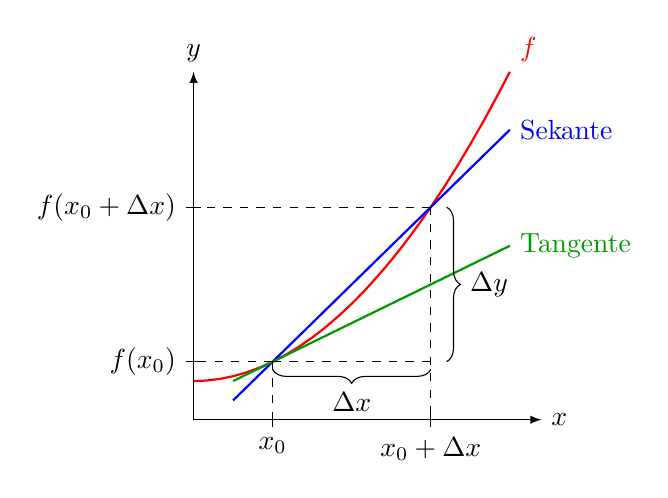
\begin{tikzpicture}
  \begin{axis}[
    width=6cm,
    height=6cm,
    xlabel={$x$},
    ylabel={$y$},
    xmin = 0, xmax = 4.4,
    ymin = 0, ymax = 9,
    axis y line=middle,
    axis x line=middle,
    xtick={\empty},
    ytick={\empty},
    xlabel style={at=(current axis.right of origin), anchor=west},
    ylabel style={at=(current axis.above origin), anchor=south},
    clip=false,
    declare function = {f(\x) = 0.5*\x^2 + 1;},
    ]
    \pgfmathsetmacro{\xo}{1};
    \pgfmathsetmacro{\Dx}{2};
    \addplot[red, domain=0:4, thick] { f(x) } node[above right] { $f$ };
    \addplot[blue, domain=0.5:4, thick] { (f(\xo+\Dx)-f(\xo))/\Dx*x - (f(\xo+\Dx)-f(\xo))/\Dx*\xo + f(\xo) } node[right] { Sekante };
    \addplot[green, domain=0.5:4, thick] { x - \xo + f(\xo) } node[right] { Tangente };
    \draw[] (axis cs:\xo,0.2) -- (axis cs:\xo,-0.2) node[below] { $x_0$ };
    \draw[] (axis cs:{\xo+\Dx},0.2) -- (axis cs:{\xo+\Dx},-0.2) node[below] { $x_0+\Delta x$ };
    \draw[dashed] (axis cs:\xo,{f(\xo)}) -- (axis cs:{\xo+\Dx},{f(\xo)});
    \draw[dashed] (axis cs:{\xo},{f(\xo)}) -- (axis cs:{\xo},0);
    \draw[dashed] (axis cs:{\xo+\Dx},{f(\xo+\Dx)}) -- (axis cs:{\xo+\Dx},0);
    \draw[dashed] (axis cs:{\xo+\Dx},{f(\xo+\Dx)}) -- (axis cs:0,{f(\xo+\Dx)});
    \draw[dashed] (axis cs:{\xo},{f(\xo)}) -- (axis cs:0,{f(\xo)});
    \draw[] (axis cs:0.1,{f(\xo)}) -- (axis cs:-0.1,{f(\xo)}) node[left] { $f(x_0)$ };
    \draw[] (axis cs:0.1,{f(\xo+\Dx)}) -- (axis cs:-0.1,{f(\xo+\Dx)}) node[left] { $f(x_0+\Delta x)$ };
    \draw[decorate,decoration={brace,amplitude=5pt}] (axis cs:{\xo+\Dx+0.2},{f(\xo+\Dx)}) -- node[right,xshift=0.5em] {$\Delta y$} (axis cs:{\xo+\Dx+0.2},{f(\xo)});
    \draw[decorate,decoration={brace,amplitude=5pt}] (axis cs:{\xo+\Dx},{f(\xo)-0.2}) -- node[below,yshift=-0.5em] {$\Delta x$} (axis cs:{\xo},{f(\xo)-0.2});
  \end{axis}
\end{tikzpicture}
\end{document}
